% Claims
% 1. Uniform elasticity is suboptimal in many cases
% 2. Workload-aware data placement increases the system performance
%    - coarse-grained: 15% for powerlaw workload distribution (common workload)
% 3. Placement strategy (to show the tradeoff)
%    - increasing color span (rainbow) → better balancing workload
%    - minimizing color span (monochromatic) → largely exploting caching locality
% 4. Hybrid placement strategy shows both advantages

\section{Introduction}
\label{sec:introduction}

In large-scale, distributed systems the dataset, which is too large
for a single node, is partitioned among the nodes.
Incoming workload (\emph{i.e.,} requests) is routed among nodes by a
load balancer.
For extreme horizontal scaling to be effective, it is necessary for
nearly all requests to be routed to a node containing the needed data
locally, which avoids unnecessary node-to-node interactions.
Consequently, data replication and data placement are components of load
balancing and have a substantial impact on system performance.
In the literature, for example,
AUTOPLACER \cite{Rodrigues2013} and MET \cite{Cruz2013}
optimize data placement to fit workload characteristics in NoSQL databases.
Replicating hotter data in storage is a common approach
to balance load \cite{Lim2010}.
In relational databases, sharding is used to distribute load
by partitioning tables to achieve effective horizontal scaling
\cite{Chang2008, george2011hbase, Lakshman2010, Adya2016, Curino2010}.


Cloud computing has changed how computing resources are used.
Before cloud computing, infrastructure is purchased and used for many
years before it is upgraded or replaced.
However, with Infrastructure as a Service (IaaS) equipment is rented
for a short time, including as short as one execution of an
application.
This shift from buying to renting greatly increases the flexibility of
infrastructure available for a given application.
Therefore, rather than tune an application to run well on a specific
machine, a cloud user instead can tune the
infrastructure to accommodate each application on each
dataset.
When an infrastructure is resized in response to changes in workloads,
it is necessary to replicate and place data partitions among nodes.
It is still unclear what are the better strategies
for this decision---prior work on data placement
does not totally address these issues~\cite{Rodrigues2013, Cruz2013, Lim2010}.


Efficient deployment of distributed systems with an
irregular workload requires both cluster sizing and
data placement.
N\"aive uniform data replication (where all data partitions have the
same number of replicas) is effective only when the workload is also
uniform---requests are equally distributed among all partitions.
\emph{Workload-aware} data placement replicates and places
partitions to match the distribution of requests in the anticipated
workload.

\begin{figure}[!htbp]
    \centering
    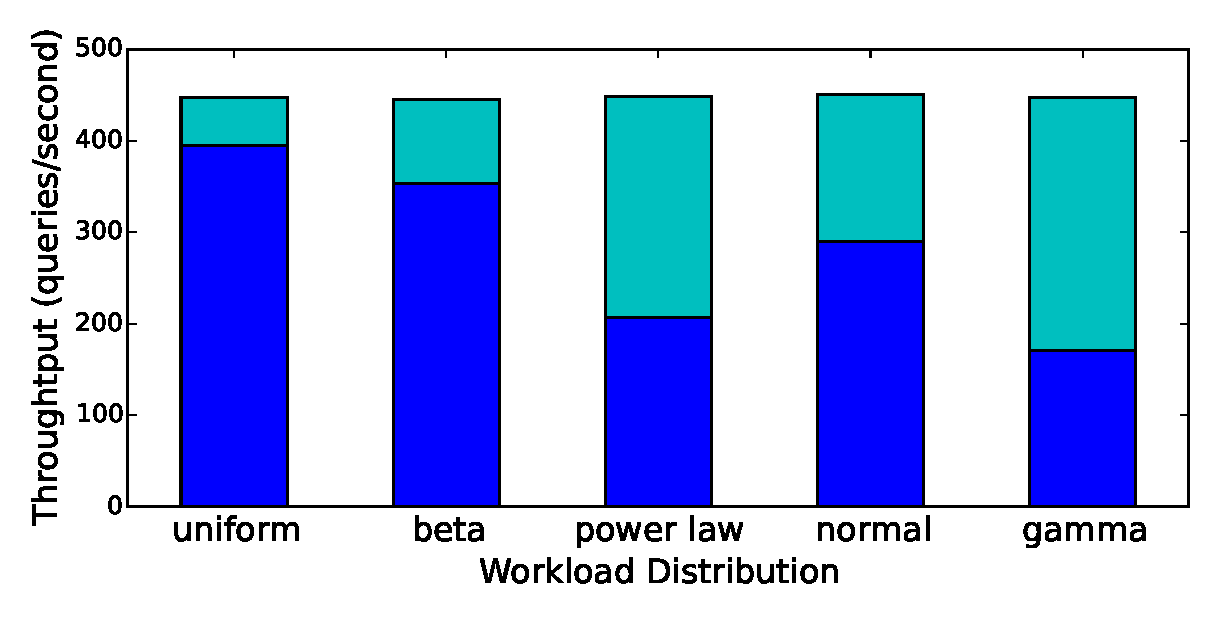
\includegraphics[width=0.8\linewidth]{figures/E34_uniform_suboptimal_tp_stacked_scdm2017.eps}
    \caption{Uniform data placement is suboptimal.
             The lower bar is the measured throughput of uniform placement while
             the upper bar is the performance loss to the idealistic placement.
(Data is a subset of data shown in
\mytable{\ref{tab:throughput_comparison_local}} on Section~\ref{sec:evaluation}.)}
    \label{fig:uniform_suboptimal}
\end{figure}

\myfigure{\ref{fig:uniform_suboptimal}} illustrates the cost of
uniform data replication on non-uniform workloads.
The results for five different workloads are presented on the $x$-axis;
the skew (degree of imbalance) in the workload increases from
left to right.
The \emph{complete} placement solution, where each node has all data,
is an idealistic upper bound on the potential gains of
matching data replication and workload.
% Uniform placement is within 10\% of ideal when the workload is
% uniform.
Because any node can process a request, new requests are sent to the
least loaded node and the performance of \emph{complete} is flat across all
workloads.
In this example, the cluster has twice the minimum capacity, so uniform
replication has two copies of each partition.
Therefore, a request must be sent to
one of the two nodes that hold the data associated
with the request.
Throughput decreases as the
workload skew increases because some nodes are over loaded and
others are under utilized.
While uniform placement achieves 88\% of ideal on uniform workload, it
is only 38\% of ideal on the highly-skewed gamma workload.
This example illustrates the need to properly \emph{replicate} and
\emph{place} data on the nodes of a cluster.


This chapter explores the three dimensions that affect data placement.
The first dimension is \emph{granularity} of data partitions.
Fine-grain (more than one partition per node) placement has costs
(overhead) and benefits (flexibility).
The second dimension is how many \emph{replicas} of each partition.
We let the anticipated demand per partition (\emph{i.e.}, the
\emph{workload}) 
determine the replication factor for each data partition.
The hotter the data, the greater the replication.
The number of data partitions influences how closely the replication
matches the workload.
However,
a coarse-grain partition (one per node) is unlikely to match the
workload.
Last, fine-grain partitioning introduces the
\emph{placement} dimension because there are several ways to distribute
the partitions among the nodes.

We present results from a simulation program that
examines these three dimensions.
We find that coarse-grain placement does not provide sufficient
flexibility to balance non-uniform loads.
A surprisingly small amount of additional partition granularity
is sufficient to load balance and obtain most benefits.
The work presents and evaluates the tradeoff between several
fine-grain placement strategies that either
increase robustness to tolerate workload deviation or
reduce storage footprint.

To further examine these conclusions, our empirical study
on an HPCC cluster\footnote{HPCC Systems is an open source
  \emph{data-analytics computer}---a highly scalable, distributed
  framework for processing and analyzing
  large datasets---supported by LexisNexis Risk Solutions at
  \url{https://hpccsystems.com/}.
}
shows that proper data replication and placement
affect system performance greatly.
The coarse-grain scheme improves system throughput by
$25\%$ and $85\%$ for the normal and power law distribution,
respectively.
A fine-grain placement strategy 
improves query throughput by $52\%$ and $105\%$.
On the most highly-skewed case, the improvement is $166\%$ increase over the
n\"aive solution.

Because data placement relies on a prediction of the upcoming
workload, which will invariably be wrong to some degree.
This chapter, therefore, considers the \emph{robustness}, which
is a measure to describe how sensitive a data placement scheme is to
slightly mis-predicted workloads, of several placement strategies.
Results show that maximizing the number of unique partitions per node
increases the robustness of a placement.